\documentclass[1p]{elsarticle_modified}
%\bibliographystyle{elsarticle-num}

%\usepackage[colorlinks]{hyperref}
%\usepackage{abbrmath_seonhwa} %\Abb, \Ascr, \Acal ,\Abf, \Afrak
\usepackage{amsfonts}
\usepackage{amssymb}
\usepackage{amsmath}
\usepackage{amsthm}
\usepackage{scalefnt}
\usepackage{amsbsy}
\usepackage{kotex}
\usepackage{caption}
\usepackage{subfig}
\usepackage{color}
\usepackage{graphicx}
\usepackage{xcolor} %% white, black, red, green, blue, cyan, magenta, yellow
\usepackage{float}
\usepackage{setspace}
\usepackage{hyperref}

\usepackage{tikz}
\usetikzlibrary{arrows}

\usepackage{multirow}
\usepackage{array} % fixed length table
\usepackage{hhline}

%%%%%%%%%%%%%%%%%%%%%
\makeatletter
\renewcommand*\env@matrix[1][\arraystretch]{%
	\edef\arraystretch{#1}%
	\hskip -\arraycolsep
	\let\@ifnextchar\new@ifnextchar
	\array{*\c@MaxMatrixCols c}}
\makeatother %https://tex.stackexchange.com/questions/14071/how-can-i-increase-the-line-spacing-in-a-matrix
%%%%%%%%%%%%%%%

\usepackage[normalem]{ulem}

\newcommand{\msout}[1]{\ifmmode\text{\sout{\ensuremath{#1}}}\else\sout{#1}\fi}
%SOURCE: \msout is \stkout macro in https://tex.stackexchange.com/questions/20609/strikeout-in-math-mode

\newcommand{\cancel}[1]{
	\ifmmode
	{\color{red}\msout{#1}}
	\else
	{\color{red}\sout{#1}}
	\fi
}

\newcommand{\add}[1]{
	{\color{blue}\uwave{#1}}
}

\newcommand{\replace}[2]{
	\ifmmode
	{\color{red}\msout{#1}}{\color{blue}\uwave{#2}}
	\else
	{\color{red}\sout{#1}}{\color{blue}\uwave{#2}}
	\fi
}

\newcommand{\Sol}{\mathcal{S}} %segment
\newcommand{\D}{D} %diagram
\newcommand{\A}{\mathcal{A}} %arc


%%%%%%%%%%%%%%%%%%%%%%%%%%%%%5 test

\def\sl{\operatorname{\textup{SL}}(2,\Cbb)}
\def\psl{\operatorname{\textup{PSL}}(2,\Cbb)}
\def\quan{\mkern 1mu \triangleright \mkern 1mu}

\theoremstyle{definition}
\newtheorem{thm}{Theorem}[section]
\newtheorem{prop}[thm]{Proposition}
\newtheorem{lem}[thm]{Lemma}
\newtheorem{ques}[thm]{Question}
\newtheorem{cor}[thm]{Corollary}
\newtheorem{defn}[thm]{Definition}
\newtheorem{exam}[thm]{Example}
\newtheorem{rmk}[thm]{Remark}
\newtheorem{alg}[thm]{Algorithm}

\newcommand{\I}{\sqrt{-1}}
\begin{document}

%\begin{frontmatter}
%
%\title{Boundary parabolic representations of knots up to 8 crossings}
%
%%% Group authors per affiliation:
%\author{Yunhi Cho} 
%\address{Department of Mathematics, University of Seoul, Seoul, Korea}
%\ead{yhcho@uos.ac.kr}
%
%
%\author{Seonhwa Kim} %\fnref{s_kim}}
%\address{Center for Geometry and Physics, Institute for Basic Science, Pohang, 37673, Korea}
%\ead{ryeona17@ibs.re.kr}
%
%\author{Hyuk Kim}
%\address{Department of Mathematical Sciences, Seoul National University, Seoul 08826, Korea}
%\ead{hyukkim@snu.ac.kr}
%
%\author{Seokbeom Yoon}
%\address{Department of Mathematical Sciences, Seoul National University, Seoul, 08826,  Korea}
%\ead{sbyoon15@snu.ac.kr}
%
%\begin{abstract}
%We find all boundary parabolic representation of knots up to 8 crossings.
%
%\end{abstract}
%\begin{keyword}
%    \MSC[2010] 57M25 
%\end{keyword}
%
%\end{frontmatter}

%\linenumbers
%\tableofcontents
%
\newcommand\colored[1]{\textcolor{white}{\rule[-0.35ex]{0.8em}{1.4ex}}\kern-0.8em\color{red} #1}%
%\newcommand\colored[1]{\textcolor{white}{ #1}\kern-2.17ex	\textcolor{white}{ #1}\kern-1.81ex	\textcolor{white}{ #1}\kern-2.15ex\color{red}#1	}

{\Large $\underline{11n_{101}~(K11n_{101})}$}

\setlength{\tabcolsep}{10pt}
\renewcommand{\arraystretch}{1.6}
\vspace{1cm}\begin{tabular}{m{100pt}>{\centering\arraybackslash}m{274pt}}
\multirow{5}{120pt}{
	\centering
	\includegraphics[width=112pt]{../../../GIT/diagram.site/Diagrams/png/717_11n_101.png}\\
\ \ \ A knot diagram\footnotemark}&
\allowdisplaybreaks
\textbf{Linearized knot diagam} \\
\cline{2-2}
 &
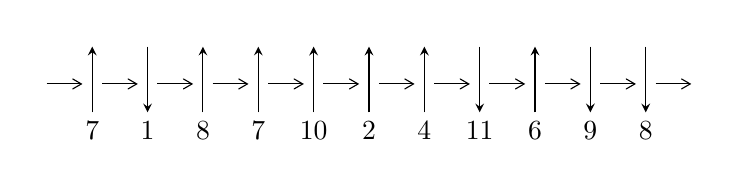
\begin{tikzpicture}[x=20pt, y=17pt]
	% nodes
	\node (C0) at (0, 0) {};
	\node (C1) at (1, 0) {};
	\node (C1U) at (1, +1) {};
	\node (C1D) at (1, -1) {7};

	\node (C2) at (2, 0) {};
	\node (C2U) at (2, +1) {};
	\node (C2D) at (2, -1) {1};

	\node (C3) at (3, 0) {};
	\node (C3U) at (3, +1) {};
	\node (C3D) at (3, -1) {8};

	\node (C4) at (4, 0) {};
	\node (C4U) at (4, +1) {};
	\node (C4D) at (4, -1) {7};

	\node (C5) at (5, 0) {};
	\node (C5U) at (5, +1) {};
	\node (C5D) at (5, -1) {10};

	\node (C6) at (6, 0) {};
	\node (C6U) at (6, +1) {};
	\node (C6D) at (6, -1) {2};

	\node (C7) at (7, 0) {};
	\node (C7U) at (7, +1) {};
	\node (C7D) at (7, -1) {4};

	\node (C8) at (8, 0) {};
	\node (C8U) at (8, +1) {};
	\node (C8D) at (8, -1) {11};

	\node (C9) at (9, 0) {};
	\node (C9U) at (9, +1) {};
	\node (C9D) at (9, -1) {6};

	\node (C10) at (10, 0) {};
	\node (C10U) at (10, +1) {};
	\node (C10D) at (10, -1) {9};

	\node (C11) at (11, 0) {};
	\node (C11U) at (11, +1) {};
	\node (C11D) at (11, -1) {8};
	\node (C12) at (12, 0) {};

	% arrows
	\draw[->,>={angle 60}]
	(C0) edge (C1) (C1) edge (C2) (C2) edge (C3) (C3) edge (C4) (C4) edge (C5) (C5) edge (C6) (C6) edge (C7) (C7) edge (C8) (C8) edge (C9) (C9) edge (C10) (C10) edge (C11) (C11) edge (C12) ;	\draw[->,>=stealth]
	(C1D) edge (C1U) (C2U) edge (C2D) (C3D) edge (C3U) (C4D) edge (C4U) (C5D) edge (C5U) (C6D) edge (C6U) (C7D) edge (C7U) (C8U) edge (C8D) (C9D) edge (C9U) (C10U) edge (C10D) (C11U) edge (C11D) ;
	\end{tikzpicture} \\
\hhline{~~} \\& 
\textbf{Solving Sequence} \\ \cline{2-2} 
 &
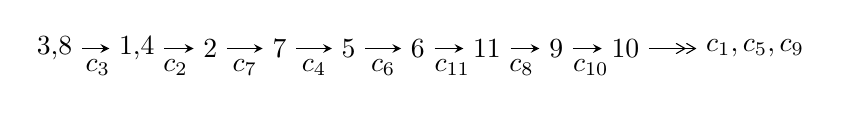
\begin{tikzpicture}[x=25pt, y=7pt]
	% node
	\node (A0) at (-1/8, 0) {3,8};
	\node (A1) at (17/16, 0) {1,4};
	\node (A2) at (17/8, 0) {2};
	\node (A3) at (25/8, 0) {7};
	\node (A4) at (33/8, 0) {5};
	\node (A5) at (41/8, 0) {6};
	\node (A6) at (49/8, 0) {11};
	\node (A7) at (57/8, 0) {9};
	\node (A8) at (65/8, 0) {10};
	\node (C1) at (1/2, -1) {$c_{3}$};
	\node (C2) at (13/8, -1) {$c_{2}$};
	\node (C3) at (21/8, -1) {$c_{7}$};
	\node (C4) at (29/8, -1) {$c_{4}$};
	\node (C5) at (37/8, -1) {$c_{6}$};
	\node (C6) at (45/8, -1) {$c_{11}$};
	\node (C7) at (53/8, -1) {$c_{8}$};
	\node (C8) at (61/8, -1) {$c_{10}$};
	\node (A9) at (10, 0) {$c_{1},c_{5},c_{9}$};

	% edge
	\draw[->,>=stealth]	
	(A0) edge (A1) (A1) edge (A2) (A2) edge (A3) (A3) edge (A4) (A4) edge (A5) (A5) edge (A6) (A6) edge (A7) (A7) edge (A8) ;
	\draw[->>,>={angle 60}]	
	(A8) edge (A9);
\end{tikzpicture} \\ 

\end{tabular} \\

\footnotetext{
The image of knot diagram is generated by the software ``\textbf{Draw programme}" developed by Andrew Bartholomew(\url{http://www.layer8.co.uk/maths/draw/index.htm\#Running-draw}), where we modified some parts for our purpose(\url{https://github.com/CATsTAILs/LinksPainter}).
}\phantom \\ \newline 
\centering \textbf{Ideals for irreducible components\footnotemark of $X_{\text{par}}$} 
 
\begin{align*}
I^u_{1}&=\langle 
- u^2+b,\;- u^{12}+u^{11}+u^9-8 u^8+6 u^7+5 u^6+2 u^5-18 u^4+5 u^3+15 u^2+8 a+u-9,\\
\phantom{I^u_{1}}&\phantom{= \langle  }u^{13}+u^{11}- u^{10}+7 u^9+3 u^7-5 u^6+8 u^5+u^4+4 u^3-2 u^2-1\rangle \\
I^u_{2}&=\langle 
-201 u^{11}-132 u^{10}+\cdots+281 b+62,\;247 u^{11}+28 u^{10}+\cdots+281 a+72,\\
\phantom{I^u_{2}}&\phantom{= \langle  }u^{12}+u^{11}+2 u^{10}+2 u^9+5 u^8+5 u^7+13 u^6+11 u^5+15 u^4+11 u^3+8 u^2+4 u+1\rangle \\
I^u_{3}&=\langle 
b+1,\;a^3- a^2 u-2 a+u,\;u^2+1\rangle \\
\\
\end{align*}
\raggedright * 3 irreducible components of $\dim_{\mathbb{C}}=0$, with total 31 representations.\\
\footnotetext{All coefficients of polynomials are rational numbers. But the coefficients are sometimes approximated in decimal forms when there is not enough margin.}
\newpage
\renewcommand{\arraystretch}{1}
\centering \section*{I. $I^u_{1}= \langle - u^2+b,\;- u^{12}+u^{11}+\cdots+8 a-9,\;u^{13}+u^{11}+\cdots-2 u^2-1 \rangle$}
\flushleft \textbf{(i) Arc colorings}\\
\begin{tabular}{m{7pt} m{180pt} m{7pt} m{180pt} }
\flushright $a_{3}=$&$\begin{pmatrix}1\\0\end{pmatrix}$ \\
\flushright $a_{8}=$&$\begin{pmatrix}0\\u\end{pmatrix}$ \\
\flushright $a_{1}=$&$\begin{pmatrix}\frac{1}{8} u^{12}-\frac{1}{8} u^{11}+\cdots-\frac{1}{8} u+\frac{9}{8}\\u^2\end{pmatrix}$ \\
\flushright $a_{4}=$&$\begin{pmatrix}1\\- u^2\end{pmatrix}$ \\
\flushright $a_{2}=$&$\begin{pmatrix}\frac{1}{8} u^{12}-\frac{1}{8} u^{11}+\cdots-\frac{1}{8} u+\frac{9}{8}\\- u^4\end{pmatrix}$ \\
\flushright $a_{7}=$&$\begin{pmatrix}- u\\u^3+u\end{pmatrix}$ \\
\flushright $a_{5}=$&$\begin{pmatrix}u^2+1\\- u^4-2 u^2\end{pmatrix}$ \\
\flushright $a_{6}=$&$\begin{pmatrix}\frac{1}{8} u^{12}+\frac{1}{8} u^{11}+\cdots-\frac{17}{8} u-\frac{1}{8}\\u^5+u^3+u\end{pmatrix}$ \\
\flushright $a_{11}=$&$\begin{pmatrix}\frac{1}{8} u^{12}-\frac{1}{8} u^{11}+\cdots-\frac{1}{8} u+\frac{9}{8}\\\frac{1}{8} u^{12}-\frac{1}{8} u^{11}+\cdots-\frac{1}{8} u+\frac{1}{8}\end{pmatrix}$ \\
\flushright $a_{9}=$&$\begin{pmatrix}\frac{7}{8} u^{12}+\frac{3}{8} u^{11}+\cdots-\frac{17}{8} u-\frac{5}{8}\\\frac{1}{2} u^{12}+\frac{1}{4} u^{10}+\cdots+\frac{1}{4} u-\frac{1}{4}\end{pmatrix}$ \\
\flushright $a_{10}=$&$\begin{pmatrix}\frac{1}{8} u^{12}+\frac{9}{8} u^{11}+\cdots+\frac{7}{8} u-\frac{13}{8}\\\frac{7}{8} u^{12}-\frac{3}{8} u^{11}+\cdots-\frac{5}{8} u-\frac{3}{8}\end{pmatrix}$\\ \flushright $a_{10}=$&$\begin{pmatrix}\frac{1}{8} u^{12}+\frac{9}{8} u^{11}+\cdots+\frac{7}{8} u-\frac{13}{8}\\\frac{7}{8} u^{12}-\frac{3}{8} u^{11}+\cdots-\frac{5}{8} u-\frac{3}{8}\end{pmatrix}$\\&\end{tabular}
\flushleft \textbf{(ii) Obstruction class $= -1$}\\~\\
\flushleft \textbf{(iii) Cusp Shapes $= 4 u^{12}+\frac{7}{2} u^{10}-\frac{7}{2} u^9+\frac{55}{2} u^8+u^7+\frac{15}{2} u^6-16 u^5+30 u^4+9 u^3+5 u^2-\frac{1}{2} u+\frac{5}{2}$}\\~\\
\newpage\renewcommand{\arraystretch}{1}
\flushleft \textbf{(iv) u-Polynomials at the component}\newline \\
\begin{tabular}{m{50pt}|m{274pt}}
Crossings & \hspace{64pt}u-Polynomials at each crossing \\
\hline $$\begin{aligned}c_{1},c_{3},c_{4}\\c_{6},c_{7}\end{aligned}$$&$\begin{aligned}
&u^{13}+u^{11}- u^{10}+7 u^9+3 u^7-5 u^6+8 u^5+u^4+4 u^3-2 u^2-1
\end{aligned}$\\
\hline $$\begin{aligned}c_{2}\end{aligned}$$&$\begin{aligned}
&u^{13}+2 u^{12}+\cdots-4 u-1
\end{aligned}$\\
\hline $$\begin{aligned}c_{5},c_{9}\end{aligned}$$&$\begin{aligned}
&u^{13}-3 u^{12}+\cdots+5 u-2
\end{aligned}$\\
\hline $$\begin{aligned}c_{8},c_{10},c_{11}\end{aligned}$$&$\begin{aligned}
&u^{13}+3 u^{12}+\cdots+5 u-4
\end{aligned}$\\
\hline
\end{tabular}\\~\\
\newpage\renewcommand{\arraystretch}{1}
\flushleft \textbf{(v) Riley Polynomials at the component}\newline \\
\begin{tabular}{m{50pt}|m{274pt}}
Crossings & \hspace{64pt}Riley Polynomials at each crossing \\
\hline $$\begin{aligned}c_{1},c_{3},c_{4}\\c_{6},c_{7}\end{aligned}$$&$\begin{aligned}
&y^{13}+2 y^{12}+\cdots-4 y-1
\end{aligned}$\\
\hline $$\begin{aligned}c_{2}\end{aligned}$$&$\begin{aligned}
&y^{13}+26 y^{12}+\cdots+12 y-1
\end{aligned}$\\
\hline $$\begin{aligned}c_{5},c_{9}\end{aligned}$$&$\begin{aligned}
&y^{13}+3 y^{12}+\cdots+5 y-4
\end{aligned}$\\
\hline $$\begin{aligned}c_{8},c_{10},c_{11}\end{aligned}$$&$\begin{aligned}
&y^{13}+15 y^{12}+\cdots+177 y-16
\end{aligned}$\\
\hline
\end{tabular}\\~\\
\newpage\flushleft \textbf{(vi) Complex Volumes and Cusp Shapes}
$$\begin{array}{c|c|c}  
\text{Solutions to }I^u_{1}& \I (\text{vol} + \sqrt{-1}CS) & \text{Cusp shape}\\
 \hline 
\begin{aligned}
u &= \phantom{-}0.871545 + 0.665952 I \\
a &= -0.145280 - 0.753872 I \\
b &= \phantom{-}0.316099 + 1.160810 I\end{aligned}
 & \phantom{-}2.81429 + 2.20167 I & \phantom{-}6.81300 - 2.37182 I \\ \hline\begin{aligned}
u &= \phantom{-}0.871545 - 0.665952 I \\
a &= -0.145280 + 0.753872 I \\
b &= \phantom{-}0.316099 - 1.160810 I\end{aligned}
 & \phantom{-}2.81429 - 2.20167 I & \phantom{-}6.81300 + 2.37182 I \\ \hline\begin{aligned}
u &= -0.745925 + 0.860258 I \\
a &= -0.294264 + 1.109470 I \\
b &= -0.183640 - 1.283380 I\end{aligned}
 & \phantom{-}1.03858 - 7.07395 I & \phantom{-}2.58380 + 8.11816 I \\ \hline\begin{aligned}
u &= -0.745925 - 0.860258 I \\
a &= -0.294264 - 1.109470 I \\
b &= -0.183640 + 1.283380 I\end{aligned}
 & \phantom{-}1.03858 + 7.07395 I & \phantom{-}2.58380 - 8.11816 I \\ \hline\begin{aligned}
u &= -0.438163 + 0.579645 I \\
a &= \phantom{-}0.727972 + 1.025400 I \\
b &= -0.144001 - 0.507958 I\end{aligned}
 & -2.29540 - 1.46021 I & -0.76105 + 4.77537 I \\ \hline\begin{aligned}
u &= -0.438163 - 0.579645 I \\
a &= \phantom{-}0.727972 - 1.025400 I \\
b &= -0.144001 + 0.507958 I\end{aligned}
 & -2.29540 + 1.46021 I & -0.76105 - 4.77537 I \\ \hline\begin{aligned}
u &= \phantom{-}0.622206\phantom{ +0.000000I} \\
a &= \phantom{-}0.441815\phantom{ +0.000000I} \\
b &= \phantom{-}0.387141\phantom{ +0.000000I}\end{aligned}
 & \phantom{-}0.957360\phantom{ +0.000000I} & \phantom{-}10.3810\phantom{ +0.000000I} \\ \hline\begin{aligned}
u &= -0.052177 + 0.598239 I \\
a &= \phantom{-}2.07278 + 0.29749 I \\
b &= -0.355168 - 0.062429 I\end{aligned}
 & \phantom{-}1.24085 + 2.67797 I & \phantom{-}5.53095 - 2.23117 I \\ \hline\begin{aligned}
u &= -0.052177 - 0.598239 I \\
a &= \phantom{-}2.07278 - 0.29749 I \\
b &= -0.355168 + 0.062429 I\end{aligned}
 & \phantom{-}1.24085 - 2.67797 I & \phantom{-}5.53095 + 2.23117 I \\ \hline\begin{aligned}
u &= -0.95082 + 1.19131 I \\
a &= -0.819335 + 0.844166 I \\
b &= -0.51516 - 2.26544 I\end{aligned}
 & \phantom{-}10.8970 - 11.1670 I & \phantom{-}4.44754 + 6.34112 I\\
 \hline 
 \end{array}$$\newpage$$\begin{array}{c|c|c}  
\text{Solutions to }I^u_{1}& \I (\text{vol} + \sqrt{-1}CS) & \text{Cusp shape}\\
 \hline 
\begin{aligned}
u &= -0.95082 - 1.19131 I \\
a &= -0.819335 - 0.844166 I \\
b &= -0.51516 + 2.26544 I\end{aligned}
 & \phantom{-}10.8970 + 11.1670 I & \phantom{-}4.44754 - 6.34112 I \\ \hline\begin{aligned}
u &= \phantom{-}1.00444 + 1.14917 I \\
a &= -0.762781 - 0.795622 I \\
b &= -0.31170 + 2.30854 I\end{aligned}
 & \phantom{-}11.32250 + 4.40088 I & \phantom{-}5.19535 - 1.84237 I \\ \hline\begin{aligned}
u &= \phantom{-}1.00444 - 1.14917 I \\
a &= -0.762781 + 0.795622 I \\
b &= -0.31170 - 2.30854 I\end{aligned}
 & \phantom{-}11.32250 - 4.40088 I & \phantom{-}5.19535 + 1.84237 I\\
 \hline 
 \end{array}$$\newpage\newpage\renewcommand{\arraystretch}{1}
\centering \section*{II. $I^u_{2}= \langle -201 u^{11}-132 u^{10}+\cdots+281 b+62,\;247 u^{11}+28 u^{10}+\cdots+281 a+72,\;u^{12}+u^{11}+\cdots+4 u+1 \rangle$}
\flushleft \textbf{(i) Arc colorings}\\
\begin{tabular}{m{7pt} m{180pt} m{7pt} m{180pt} }
\flushright $a_{3}=$&$\begin{pmatrix}1\\0\end{pmatrix}$ \\
\flushright $a_{8}=$&$\begin{pmatrix}0\\u\end{pmatrix}$ \\
\flushright $a_{1}=$&$\begin{pmatrix}-0.879004 u^{11}-0.0996441 u^{10}+\cdots-4.62633 u-0.256228\\0.715302 u^{11}+0.469751 u^{10}+\cdots+2.23843 u-0.220641\end{pmatrix}$ \\
\flushright $a_{4}=$&$\begin{pmatrix}1\\- u^2\end{pmatrix}$ \\
\flushright $a_{2}=$&$\begin{pmatrix}-1.59431 u^{11}-0.569395 u^{10}+\cdots-6.86477 u-1.03559\\1.23132 u^{11}+0.868327 u^{10}+\cdots+4.74377 u+0.804270\end{pmatrix}$ \\
\flushright $a_{7}=$&$\begin{pmatrix}- u\\u^3+u\end{pmatrix}$ \\
\flushright $a_{5}=$&$\begin{pmatrix}u^2+1\\- u^4-2 u^2\end{pmatrix}$ \\
\flushright $a_{6}=$&$\begin{pmatrix}-0.754448 u^{11}-0.555160 u^{10}+\cdots-4.91815 u-3.28470\\0.661922 u^{11}-0.192171 u^{10}+\cdots+0.220641 u+0.362989\end{pmatrix}$ \\
\flushright $a_{11}=$&$\begin{pmatrix}-0.879004 u^{11}-0.0996441 u^{10}+\cdots-4.62633 u-0.256228\\1.43060 u^{11}+0.939502 u^{10}+\cdots+4.47687 u+0.558719\end{pmatrix}$ \\
\flushright $a_{9}=$&$\begin{pmatrix}-1.77936 u^{11}-1.06406 u^{10}+\cdots-10.2598 u-4.87900\\1.27046 u^{11}+0.953737 u^{10}+\cdots+6.42349 u+2.30961\end{pmatrix}$ \\
\flushright $a_{10}=$&$\begin{pmatrix}- u^2-1\\1.43060 u^{11}+0.939502 u^{10}+\cdots+4.47687 u+1.55872\end{pmatrix}$\\ \flushright $a_{10}=$&$\begin{pmatrix}- u^2-1\\1.43060 u^{11}+0.939502 u^{10}+\cdots+4.47687 u+1.55872\end{pmatrix}$\\&\end{tabular}
\flushleft \textbf{(ii) Obstruction class $= -1$}\\~\\
\flushleft \textbf{(iii) Cusp Shapes $= \frac{212}{281} u^{11}+\frac{1280}{281} u^{10}+\frac{404}{281} u^9+\frac{1208}{281} u^8+\frac{1568}{281} u^7+\frac{4548}{281} u^6+\frac{3124}{281} u^5+\frac{10520}{281} u^4+\frac{2840}{281} u^3+\frac{6608}{281} u^2+\frac{1944}{281} u+\frac{1766}{281}$}\\~\\
\newpage\renewcommand{\arraystretch}{1}
\flushleft \textbf{(iv) u-Polynomials at the component}\newline \\
\begin{tabular}{m{50pt}|m{274pt}}
Crossings & \hspace{64pt}u-Polynomials at each crossing \\
\hline $$\begin{aligned}c_{1},c_{3},c_{4}\\c_{6},c_{7}\end{aligned}$$&$\begin{aligned}
&u^{12}+u^{11}+\cdots+4 u+1
\end{aligned}$\\
\hline $$\begin{aligned}c_{2}\end{aligned}$$&$\begin{aligned}
&u^{12}+3 u^{11}+\cdots+6 u^2+1
\end{aligned}$\\
\hline $$\begin{aligned}c_{5},c_{9}\end{aligned}$$&$\begin{aligned}
&(u^6+u^5+u^4+2 u^2+u+1)^2
\end{aligned}$\\
\hline $$\begin{aligned}c_{8},c_{10},c_{11}\end{aligned}$$&$\begin{aligned}
&(u^6+u^5+5 u^4+4 u^3+6 u^2+3 u+1)^2
\end{aligned}$\\
\hline
\end{tabular}\\~\\
\newpage\renewcommand{\arraystretch}{1}
\flushleft \textbf{(v) Riley Polynomials at the component}\newline \\
\begin{tabular}{m{50pt}|m{274pt}}
Crossings & \hspace{64pt}Riley Polynomials at each crossing \\
\hline $$\begin{aligned}c_{1},c_{3},c_{4}\\c_{6},c_{7}\end{aligned}$$&$\begin{aligned}
&y^{12}+3 y^{11}+\cdots+6 y^2+1
\end{aligned}$\\
\hline $$\begin{aligned}c_{2}\end{aligned}$$&$\begin{aligned}
&y^{12}+11 y^{11}+\cdots+12 y+1
\end{aligned}$\\
\hline $$\begin{aligned}c_{5},c_{9}\end{aligned}$$&$\begin{aligned}
&(y^6+y^5+5 y^4+4 y^3+6 y^2+3 y+1)^2
\end{aligned}$\\
\hline $$\begin{aligned}c_{8},c_{10},c_{11}\end{aligned}$$&$\begin{aligned}
&(y^6+9 y^5+29 y^4+40 y^3+22 y^2+3 y+1)^2
\end{aligned}$\\
\hline
\end{tabular}\\~\\
\newpage\flushleft \textbf{(vi) Complex Volumes and Cusp Shapes}
$$\begin{array}{c|c|c}  
\text{Solutions to }I^u_{2}& \I (\text{vol} + \sqrt{-1}CS) & \text{Cusp shape}\\
 \hline 
\begin{aligned}
u &= \phantom{-}0.276186 + 0.937280 I \\
a &= \phantom{-}1.096930 + 0.475717 I \\
b &= \phantom{-}0.126264 - 0.186282 I\end{aligned}
 & \phantom{-}1.35295 + 2.65597 I & \phantom{-}5.58115 - 3.39809 I \\ \hline\begin{aligned}
u &= \phantom{-}0.276186 - 0.937280 I \\
a &= \phantom{-}1.096930 - 0.475717 I \\
b &= \phantom{-}0.126264 + 0.186282 I\end{aligned}
 & \phantom{-}1.35295 - 2.65597 I & \phantom{-}5.58115 + 3.39809 I \\ \hline\begin{aligned}
u &= -0.247920 + 0.814674 I \\
a &= -0.293452 + 0.484072 I \\
b &= -1.372270 + 0.172983 I\end{aligned}
 & -3.54796 - 1.10871 I & \phantom{-}0.46385 + 6.18117 I \\ \hline\begin{aligned}
u &= -0.247920 - 0.814674 I \\
a &= -0.293452 - 0.484072 I \\
b &= -1.372270 - 0.172983 I\end{aligned}
 & -3.54796 + 1.10871 I & \phantom{-}0.46385 - 6.18117 I \\ \hline\begin{aligned}
u &= -0.073688 + 1.173750 I \\
a &= \phantom{-}0.321857 + 0.253794 I \\
b &= -0.602229 + 0.403948 I\end{aligned}
 & -3.54796 + 1.10871 I & \phantom{-}0.46385 - 6.18117 I \\ \hline\begin{aligned}
u &= -0.073688 - 1.173750 I \\
a &= \phantom{-}0.321857 - 0.253794 I \\
b &= -0.602229 - 0.403948 I\end{aligned}
 & -3.54796 - 1.10871 I & \phantom{-}0.46385 + 6.18117 I \\ \hline\begin{aligned}
u &= -1.18584 + 0.84722 I \\
a &= \phantom{-}0.727937 - 0.977012 I \\
b &= \phantom{-}0.46202 + 2.13527 I\end{aligned}
 & \phantom{-}12.06460 + 3.42721 I & \phantom{-}5.95500 - 2.25224 I \\ \hline\begin{aligned}
u &= -1.18584 - 0.84722 I \\
a &= \phantom{-}0.727937 + 0.977012 I \\
b &= \phantom{-}0.46202 - 2.13527 I\end{aligned}
 & \phantom{-}12.06460 - 3.42721 I & \phantom{-}5.95500 + 2.25224 I \\ \hline\begin{aligned}
u &= \phantom{-}1.15037 + 0.92808 I \\
a &= \phantom{-}0.735494 + 0.949873 I \\
b &= \phantom{-}0.68843 - 2.00934 I\end{aligned}
 & \phantom{-}12.06460 + 3.42721 I & \phantom{-}5.95500 - 2.25224 I \\ \hline\begin{aligned}
u &= \phantom{-}1.15037 - 0.92808 I \\
a &= \phantom{-}0.735494 - 0.949873 I \\
b &= \phantom{-}0.68843 + 2.00934 I\end{aligned}
 & \phantom{-}12.06460 - 3.42721 I & \phantom{-}5.95500 + 2.25224 I\\
 \hline 
 \end{array}$$\newpage$$\begin{array}{c|c|c}  
\text{Solutions to }I^u_{2}& \I (\text{vol} + \sqrt{-1}CS) & \text{Cusp shape}\\
 \hline 
\begin{aligned}
u &= -0.419110 + 0.222236 I \\
a &= \phantom{-}1.41124 - 2.01830 I \\
b &= -0.802215 + 0.517727 I\end{aligned}
 & \phantom{-}1.35295 + 2.65597 I & \phantom{-}5.58115 - 3.39809 I \\ \hline\begin{aligned}
u &= -0.419110 - 0.222236 I \\
a &= \phantom{-}1.41124 + 2.01830 I \\
b &= -0.802215 - 0.517727 I\end{aligned}
 & \phantom{-}1.35295 - 2.65597 I & \phantom{-}5.58115 + 3.39809 I\\
 \hline 
 \end{array}$$\newpage\newpage\renewcommand{\arraystretch}{1}
\centering \section*{III. $I^u_{3}= \langle b+1,\;a^3- a^2 u-2 a+u,\;u^2+1 \rangle$}
\flushleft \textbf{(i) Arc colorings}\\
\begin{tabular}{m{7pt} m{180pt} m{7pt} m{180pt} }
\flushright $a_{3}=$&$\begin{pmatrix}1\\0\end{pmatrix}$ \\
\flushright $a_{8}=$&$\begin{pmatrix}0\\u\end{pmatrix}$ \\
\flushright $a_{1}=$&$\begin{pmatrix}a\\-1\end{pmatrix}$ \\
\flushright $a_{4}=$&$\begin{pmatrix}1\\1\end{pmatrix}$ \\
\flushright $a_{2}=$&$\begin{pmatrix}a+1\\-1\end{pmatrix}$ \\
\flushright $a_{7}=$&$\begin{pmatrix}- u\\0\end{pmatrix}$ \\
\flushright $a_{5}=$&$\begin{pmatrix}0\\1\end{pmatrix}$ \\
\flushright $a_{6}=$&$\begin{pmatrix}a u\\- u\end{pmatrix}$ \\
\flushright $a_{11}=$&$\begin{pmatrix}a\\a-1\end{pmatrix}$ \\
\flushright $a_{9}=$&$\begin{pmatrix}- a^2 u\\- a^2 u+a u+u\end{pmatrix}$ \\
\flushright $a_{10}=$&$\begin{pmatrix}- a^2 u- a+u\\- a^2 u+a^2+u-1\end{pmatrix}$\\ \flushright $a_{10}=$&$\begin{pmatrix}- a^2 u- a+u\\- a^2 u+a^2+u-1\end{pmatrix}$\\&\end{tabular}
\flushleft \textbf{(ii) Obstruction class $= 1$}\\~\\
\flushleft \textbf{(iii) Cusp Shapes $= 4 a^2-4 a u-8$}\\~\\
\newpage\renewcommand{\arraystretch}{1}
\flushleft \textbf{(iv) u-Polynomials at the component}\newline \\
\begin{tabular}{m{50pt}|m{274pt}}
Crossings & \hspace{64pt}u-Polynomials at each crossing \\
\hline $$\begin{aligned}c_{1},c_{3},c_{4}\\c_{6},c_{7}\end{aligned}$$&$\begin{aligned}
&(u^2+1)^3
\end{aligned}$\\
\hline $$\begin{aligned}c_{2}\end{aligned}$$&$\begin{aligned}
&(u+1)^6
\end{aligned}$\\
\hline $$\begin{aligned}c_{5},c_{9}\end{aligned}$$&$\begin{aligned}
&u^6+u^4+2 u^2+1
\end{aligned}$\\
\hline $$\begin{aligned}c_{8}\end{aligned}$$&$\begin{aligned}
&(u^3- u^2+2 u-1)^2
\end{aligned}$\\
\hline $$\begin{aligned}c_{10},c_{11}\end{aligned}$$&$\begin{aligned}
&(u^3+u^2+2 u+1)^2
\end{aligned}$\\
\hline
\end{tabular}\\~\\
\newpage\renewcommand{\arraystretch}{1}
\flushleft \textbf{(v) Riley Polynomials at the component}\newline \\
\begin{tabular}{m{50pt}|m{274pt}}
Crossings & \hspace{64pt}Riley Polynomials at each crossing \\
\hline $$\begin{aligned}c_{1},c_{3},c_{4}\\c_{6},c_{7}\end{aligned}$$&$\begin{aligned}
&(y+1)^6
\end{aligned}$\\
\hline $$\begin{aligned}c_{2}\end{aligned}$$&$\begin{aligned}
&(y-1)^6
\end{aligned}$\\
\hline $$\begin{aligned}c_{5},c_{9}\end{aligned}$$&$\begin{aligned}
&(y^3+y^2+2 y+1)^2
\end{aligned}$\\
\hline $$\begin{aligned}c_{8},c_{10},c_{11}\end{aligned}$$&$\begin{aligned}
&(y^3+3 y^2+2 y-1)^2
\end{aligned}$\\
\hline
\end{tabular}\\~\\
\newpage\flushleft \textbf{(vi) Complex Volumes and Cusp Shapes}
$$\begin{array}{c|c|c}  
\text{Solutions to }I^u_{3}& \I (\text{vol} + \sqrt{-1}CS) & \text{Cusp shape}\\
 \hline 
\begin{aligned}
u &= \phantom{-0.000000 -}1.000000 I \\
a &= \phantom{-}1.307140 + 0.215080 I \\
b &= -1.00000\phantom{ +0.000000I}\end{aligned}
 & -0.26574 + 2.82812 I & -0.49024 - 2.97945 I \\ \hline\begin{aligned}
u &= \phantom{-0.000000 -}1.000000 I \\
a &= -1.307140 + 0.215080 I \\
b &= -1.00000\phantom{ +0.000000I}\end{aligned}
 & -0.26574 - 2.82812 I & -0.49024 + 2.97945 I \\ \hline\begin{aligned}
u &= \phantom{-0.000000 -}1.000000 I \\
a &= \phantom{-0.000000 -}0.569840 I \\
b &= -1.00000\phantom{ +0.000000I}\end{aligned}
 & -4.40332\phantom{ +0.000000I} & -7.01950\phantom{ +0.000000I} \\ \hline\begin{aligned}
u &= \phantom{-0.000000 } -1.000000 I \\
a &= -1.307140 - 0.215080 I \\
b &= -1.00000\phantom{ +0.000000I}\end{aligned}
 & -0.26574 - 2.82812 I & -0.49024 + 2.97945 I \\ \hline\begin{aligned}
u &= \phantom{-0.000000 } -1.000000 I \\
a &= \phantom{-}1.307140 - 0.215080 I \\
b &= -1.00000\phantom{ +0.000000I}\end{aligned}
 & -0.26574 + 2.82812 I & -0.49024 - 2.97945 I \\ \hline\begin{aligned}
u &= \phantom{-0.000000 } -1.000000 I \\
a &= \phantom{-0.000000 } -0.569840 I \\
b &= -1.00000\phantom{ +0.000000I}\end{aligned}
 & -4.40332\phantom{ +0.000000I} & -7.01950\phantom{ +0.000000I}\\
 \hline 
 \end{array}$$\newpage
\newpage\renewcommand{\arraystretch}{1}
\centering \section*{ IV. u-Polynomials}
\begin{tabular}{m{50pt}|m{274pt}}
Crossings & \hspace{64pt}u-Polynomials at each crossing \\
\hline $$\begin{aligned}c_{1},c_{3},c_{4}\\c_{6},c_{7}\end{aligned}$$&$\begin{aligned}
&((u^2+1)^3)(u^{12}+u^{11}+\cdots+4 u+1)\\
&\cdot(u^{13}+u^{11}- u^{10}+7 u^9+3 u^7-5 u^6+8 u^5+u^4+4 u^3-2 u^2-1)
\end{aligned}$\\
\hline $$\begin{aligned}c_{2}\end{aligned}$$&$\begin{aligned}
&((u+1)^6)(u^{12}+3 u^{11}+\cdots+6 u^2+1)(u^{13}+2 u^{12}+\cdots-4 u-1)
\end{aligned}$\\
\hline $$\begin{aligned}c_{5},c_{9}\end{aligned}$$&$\begin{aligned}
&(u^6+u^4+2 u^2+1)(u^6+u^5+u^4+2 u^2+u+1)^2\\
&\cdot(u^{13}-3 u^{12}+\cdots+5 u-2)
\end{aligned}$\\
\hline $$\begin{aligned}c_{8}\end{aligned}$$&$\begin{aligned}
&(u^3- u^2+2 u-1)^2(u^6+u^5+5 u^4+4 u^3+6 u^2+3 u+1)^2\\
&\cdot(u^{13}+3 u^{12}+\cdots+5 u-4)
\end{aligned}$\\
\hline $$\begin{aligned}c_{10},c_{11}\end{aligned}$$&$\begin{aligned}
&(u^3+u^2+2 u+1)^2(u^6+u^5+5 u^4+4 u^3+6 u^2+3 u+1)^2\\
&\cdot(u^{13}+3 u^{12}+\cdots+5 u-4)
\end{aligned}$\\
\hline
\end{tabular}\newpage\renewcommand{\arraystretch}{1}
\centering \section*{ V. Riley Polynomials}
\begin{tabular}{m{50pt}|m{274pt}}
Crossings & \hspace{64pt}Riley Polynomials at each crossing \\
\hline $$\begin{aligned}c_{1},c_{3},c_{4}\\c_{6},c_{7}\end{aligned}$$&$\begin{aligned}
&((y+1)^6)(y^{12}+3 y^{11}+\cdots+6 y^2+1)(y^{13}+2 y^{12}+\cdots-4 y-1)
\end{aligned}$\\
\hline $$\begin{aligned}c_{2}\end{aligned}$$&$\begin{aligned}
&((y-1)^6)(y^{12}+11 y^{11}+\cdots+12 y+1)(y^{13}+26 y^{12}+\cdots+12 y-1)
\end{aligned}$\\
\hline $$\begin{aligned}c_{5},c_{9}\end{aligned}$$&$\begin{aligned}
&(y^3+y^2+2 y+1)^2(y^6+y^5+5 y^4+4 y^3+6 y^2+3 y+1)^2\\
&\cdot(y^{13}+3 y^{12}+\cdots+5 y-4)
\end{aligned}$\\
\hline $$\begin{aligned}c_{8},c_{10},c_{11}\end{aligned}$$&$\begin{aligned}
&(y^3+3 y^2+2 y-1)^2(y^6+9 y^5+29 y^4+40 y^3+22 y^2+3 y+1)^2\\
&\cdot(y^{13}+15 y^{12}+\cdots+177 y-16)
\end{aligned}$\\
\hline
\end{tabular}
\vskip 2pc
\end{document}